\documentclass{minimal}
\usepackage{tikz}
\usetikzlibrary{trees}
\begin{document}
\tikzstyle{every node}=[draw=black,thick,anchor=west]
\tikzstyle{selected}=[draw=red,fill=red!30]
\tikzstyle{optional}=[dashed,fill=gray!50]
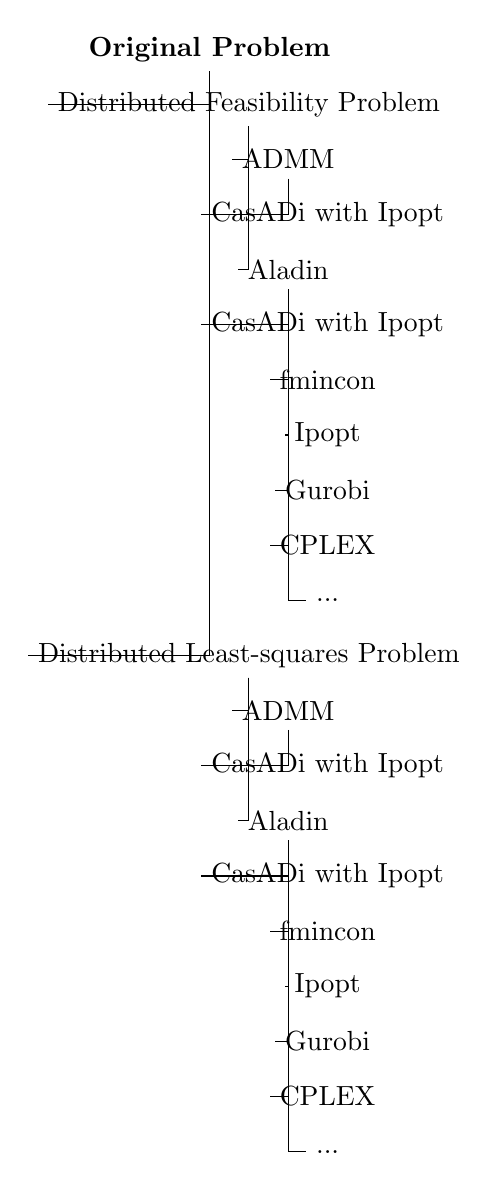
\begin{tikzpicture}[%
  grow via three points={one child at (0.5,-0.7) and
  two children at (0.5,-0.7) and (0.5,-1.4)},
  edge from parent path={(\tikzparentnode.south) |- (\tikzchildnode.west)}]
  \node {\textbf{Original Problem}}
    child { node {Distributed Feasibility Problem}
        child { node{ADMM}
            child { node{CasADi with Ipopt}}
        }
        child [missing] {}
        child { node{Aladin}
            child { node{CasADi with Ipopt}}
            child { node{fmincon}}
            child { node{Ipopt}}
            child { node{Gurobi}}
            child { node{CPLEX}}
            child { node{...}}
        }
    }
    child [missing] {}
    child [missing] {}
    child [missing] {}
    child [missing] {}
    child [missing] {}
    child [missing] {}
    child [missing] {}
    child [missing] {}
    child [missing] {}
    child { node {Distributed Least-squares Problem}
        child { node{ADMM}
            child { node{CasADi with Ipopt}}
        }
        child [missing] {}
        child { node{Aladin}
            child { node{CasADi with Ipopt}}
            child { node{fmincon}}
            child { node{Ipopt}}
            child { node{Gurobi}}
            child { node{CPLEX}}
            child { node{...}}
        }
    };
\end{tikzpicture}
\end{document}
